\newpage
\section{METHODOLOGY}

\subsection{System Block Diagram}

\begin{figure}[h]
        \centering
        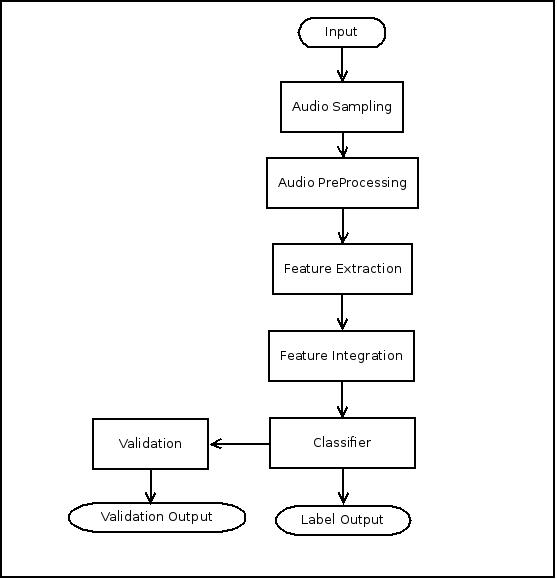
\includegraphics[width=100mm]{resources/generalworkflow}
        \caption{General workflow}
\end{figure}

\subsection{Audio Sampling}
First of all to extract any features from a audio, samples are first taken out of it. Theses samples are then fine tuned to the correct audio format. This process involves converting to mono signals if they are stereo and adjusting bit depths if it is deemed to be necessary. Sample extraction and audio format is correction is achieved through the java sound API.\\
Audio Sampling is then followed by audio framing and then a hamming window is used. Windows are necessary because whenever we do a finite Fourier transform, it is implicitly being applied to an infinitely repeating signal. So, for instance, if the start and end of a finite sample doesn’t match then that will look just like a discontinuity in the signal, and show up as lots of high-frequency nonsense in the Fourier transform, which is harmful. If the sample happens to be a perfect sinusoid but with an integer number of periods then it doesn't fit exactly into the finite sample and the FT will show appreciable energy in all sorts of places nowhere near the real frequency. Windowing the data makes sure that the ends match up while keeping everything reasonably smooth.\\
\\
Pre processing the audio signal involves the following sub steps:

\begin{itemize}

        \item Sampling the audio and fixing the audio format (Bit depth, number of channels etc) 

        \item Audio framing to carry out feature extraction in each frame individually. 

        \item Finally the use a hamming window to minimize the signal side lobe (unwanted radiation). Thus improving the quality or harmonics of the sound

\end{itemize}

Feature extraction involves the calculation of the following features:Root Mean Square(RMS), Compactness, MFCC, Rhythm, Pitch, Zero Crossing, Spectral variability, Spectral roll off point, Spectral centroid and Spectral flux. 
These features are extracted using the algorithms described in the previous chapter.\\
\\
Feature integration involves the use of various measures of performance such as precision, recall and F measure to determine which feature is the best to calculate the genre/arousal/valence of an audio signal.  
So, using the accuracy produced by each feature when used in the SVM classifier, we select the best features, or a combination of features for the particular classification.
We then integrate the features together by simply appending them.\\
\\
Finally in the classification part of the system, we utilize two different types of classifiers, Artificial Neural networks and Support Vector machines to classify the audio signals and find the proper label for each based on genre/arousal/valence.\\
\\
Validation is done when building the model. We use k-fold cross-validation with k=10 to validate the classifier.
Obviously, this step is not done in the workflow of the final product.\\

